\documentclass{article}
\usepackage[utf8]{inputenc}
\usepackage{setspace}
\onehalfspacing
\usepackage{hyperref}
\usepackage{graphicx}
\usepackage{float}
\usepackage{natbib}
\usepackage{graphicx}
\usepackage{geometry}
\usepackage{eurosym}
\usepackage{enumitem}
\usepackage{amsmath}

\geometry{top=100px, bottom=100px, left=75px, right=75px}

\begin{document}
\begin{titlepage}
    \begin{center}
        \vspace*{1cm}
        
        
        \Huge
        \textbf{Bases de données}
        
        \Huge
        \textbf{INFO-H303}
        
        \vspace{0.5cm}
        \LARGE
        {Trottinettes}
        
        \vspace{0.5cm}
        
        
        \vspace{1.5cm}
        

        \Large{Préparation et ajustement:}
        
        \vspace{0.25cm}
        
        \textbf{BAKKALI Yahya (000445166) \\}
        \textbf{FALLAHI Amirmohammad (000460073) \\}
        \textbf{HAUWAERT Maxime (000461714) \\}
        
        \vspace{0.25cm}
        
        \LARGE
        {(Groupe AA)}
        
        \vspace{0.8cm}
        
        Mars/Avril/Mai 2019
        
        \vspace{0.8cm}

        \textsc{Université Libre de Bruxelles (ULB)}
        
        
    \end{center}
\end{titlepage}

\section{Introduction}
    Le but du projet est de modéliser un programme qui gère un ensemble de trottinettes électriques se déplaçant dans Bruxelles. Les trottinettes peuvent être déposées sur le bord de la route. Pour réaliser cela on commence par modéliser le problème en utilisant un diagramme entité-association et une traduction relationnelle pour pouvoir implémenter et  manipuler la base de données correspondante.
    
\section{Le diagramme entité-association et ses contraintes }

    \subsection{Le diagramme entité-association}
        \begin{figure} [H]
            \centering
            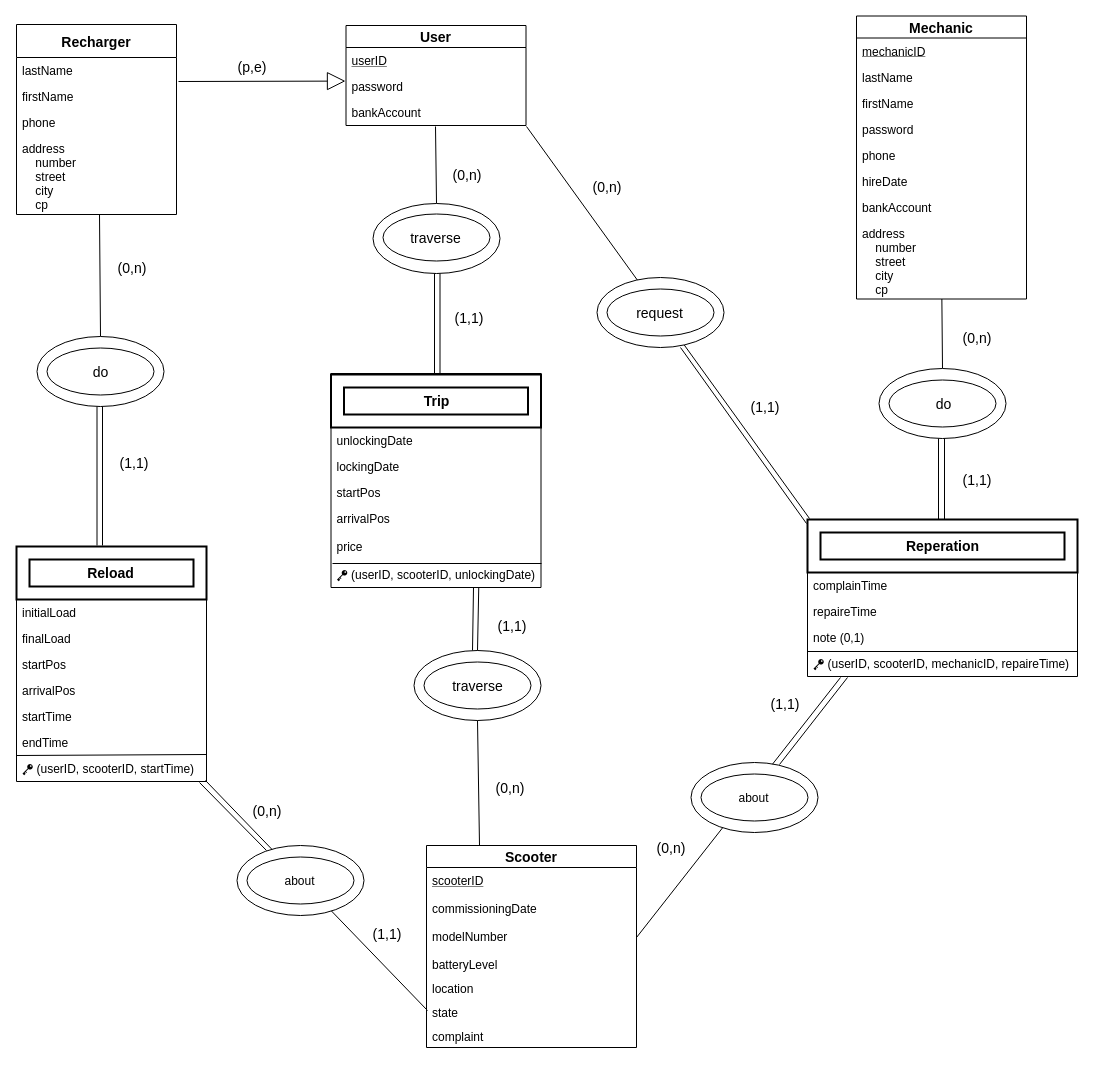
\includegraphics[width=13cm]{images/v_2.png}
            \caption{Le diagramme entité-association modélisant le problème}
        \end{figure}
        
        
     \subsection{Les contraintes du diagramme entité-association}
        \begin{enumerate}
            \item {Pour chaque trajet, la société doit bloquer une partie de l'argent du compte de l'utilisateur en cas de dégradation ou de vol.}
            \item {A chaque déverrouillage d'une trottinette, la société doit retirer 1\euro\ du compte de l'utilisateur.}   
            \item {A chaque minute d'utilisation d'une trottinette, la société doit retirer 0.15\euro\ du compte de l'utilisateur.}
            \item {Si la durée d'un trajet dépasse une heure, le coût sera réduit à 6.5\euro\ par heure.}
            \item {Si le trajet dépasse un jour, le coût sera réduit à 36\euro\ par jour.}
            \item {L'utilisateur qui charge une trottinette doit la prendre après 22h, puis, la redéposer quelque part avant 7h du matin.}
            \item {Pour chaque niveau de charge rechargé, l'utilisateur recevra 2\euro\ .}
            \item {Toutes les réparations doivent être effectuées entre 22h et 7h.}
            \item {Dans une séance de rechargement, l'état de charge du début doit être un état plus faible que l'état de fin.}
            %\item {Dans un trajet, l'état de charge du début doit être le même ou un état plus important que l'état de fin.}
            \item{Le moment de déverouillage doit être plus petit que le moment de verouillage.}
            \item{Le moment de dépot de la plainte doit être plus petit que le moment de réparation.}
        \end{enumerate}


\section{La traduction relationnelle et ses contraintes}
    \subsection{Traduction du modèle entité-association vers le modèle relationnel}

\textbf{\\Scooter}(\underline{scooterID}, commissioningDate, modelNumber, batteryLevel, location, state, complaint)
\\\\
\textbf{Mechanic}(\underline{mechanicID},lastName, firstName, password, phone, hireDate, bankAccount, adrsNumber, adrsStreet, adrsCity, adrsCp)
\\\\
\textbf{User}(\underline{userID}, password, bankAccount)
\\\\
\textbf{Recharger}(\underline{userID}, lastName, firstName, phone, adrsNumber, adrsStreet, adrsCity, adrsCp) \\
userID référence User.userID
\\\\
\textbf{Reperation}(\underline{userID, scooterID, mechanicID, repaireTime}, complainTime, repaireTime, note) \\
userID référence User.userID\\
scooterID référence Scooter.scooterID\\
mechanicID référence Mechanic.mechanicID
\\\\
\textbf{Reload}(\underline{userID, scooterID, startTime}, initialLoad, finalLoad, startPos, arrivalPos, startTime, endTime) \\
userID référence User.userID\\
scooterID référence Scooter.scooterID\\
\\
\textbf{Trip}(\underline{userID, scooterID, unlockingDate}, unlockingDate, lockingDate, startPos, arrivalPos, price) \\
userID référence User.userID\\
scooterID référence Scooter.scooterID\\
\\

    
    \subsection{Les contraintes de la traduction relationnelle}
        \begin{enumerate}
            \item {Reload.initialLoad $\leq$ Reload.finalLoad}
            \item {1 $\leq$ Scooter.batteryLevel $\leq$ 4}
            %\item {Après une trajet Scooter.batteryLevel \textless\ Scooter.batteryLevel avant la trajet }
            \item { Trip.unlockingDate \textless\ Trip.lockingDate}
            \item {Reperation.complainTime \textless\ Reperation.repaireTime}
        \end{enumerate}

\section{Les hypothèses}
        \begin{enumerate}
            \item {Un utilisateur ne peut utiliser qu'une et une seule trottinette à la fois.}
            \item {Une réperation ne concerne qu'une seule trottinette.}
        \end{enumerate}

\end{document}
